\documentclass{beamer}
\usepackage{amsmath}
\usepackage[english]{babel} %set language; note: after changing this, you need to delete all auxiliary files to recompile
\usepackage[utf8]{inputenc} %define file encoding; latin1 is the other often used option
\usepackage{csquotes} % provides context sensitive quotation facilities
\usepackage{graphicx} %allows for inserting figures
\usepackage{booktabs} % for table formatting without vertical lines
\usepackage{textcomp} % allow for example using the Euro sign with \texteuro
\usepackage{stackengine}
\usepackage{wasysym}
\usepackage{tikzsymbols}
\usepackage{textcomp}
\newcommand{\bubblethis}[2]{
        \tikz[remember picture,baseline]{\node[anchor=base,inner sep=0,outer sep=0]%
        (#1) {\underline{#1}};\node[overlay,cloud callout,callout relative pointer={(0.2cm,-0.7cm)},%
        aspect=2.5,fill=yellow!90] at ($(#1.north)+(-0.5cm,1.6cm)$) {#2};}%
    }%
\tikzset{face/.style={shape=circle,minimum size=4ex,shading=radial,outer sep=0pt,
        inner color=white!50!yellow,outer color= yellow!70!orange}}
%% Some commands to make the code easier
\newcommand{\emoticon}[1][]{%
  \node[face,#1] (emoticon) {};
  %% The eyes are fixed.
  \draw[fill=white] (-1ex,0ex) ..controls (-0.5ex,0.2ex)and(0.5ex,0.2ex)..
        (1ex,0.0ex) ..controls ( 1.5ex,1.5ex)and( 0.2ex,1.7ex)..
        (0ex,0.4ex) ..controls (-0.2ex,1.7ex)and(-1.5ex,1.5ex)..
        (-1ex,0ex)--cycle;}
\newcommand{\pupils}{
  %% standard pupils
  \fill[shift={(0.5ex,0.5ex)},rotate=80] 
       (0,0) ellipse (0.3ex and 0.15ex);
  \fill[shift={(-0.5ex,0.5ex)},rotate=100] 
       (0,0) ellipse (0.3ex and 0.15ex);}

\newcommand{\emoticonname}[1]{
  \node[below=1ex of emoticon,font=\footnotesize,
        minimum width=4cm]{#1};}
\usepackage{scalerel}
\usetikzlibrary{positioning}
\usepackage{xcolor,amssymb}
\newcommand\dangersignb[1][2ex]{%
  \scaleto{\stackengine{0.3pt}{\scalebox{1.1}[.9]{%
  \color{red}$\blacktriangle$}}{\tiny\bfseries !}{O}{c}{F}{F}{L}}{#1}%
}
\newcommand\dangersignw[1][2ex]{%
  \scaleto{\stackengine{0.3pt}{\scalebox{1.1}[.9]{%
  \color{red}$\blacktriangle$}}{\color{white}\tiny\bfseries !}{O}{c}{F}{F}{L}}{#1}%
}
\usepackage{fontawesome} % Social Icons
\usepackage{epstopdf} % allow embedding eps-figures
\usepackage{tikz} % allows drawing figures
\usepackage{amsmath,amssymb,amsthm} %advanced math facilities
\usepackage{lmodern} %uses font that support italic and bold at the same time
\usepackage{hyperref}
\usepackage{tikz}

\usepackage{tcolorbox}

\usefonttheme[onlymath]{serif} %set math font to serif ones

\definecolor{beamerblue}{rgb}{0.2,0.2,0.7} %define beamerblue color for later use

%%% defines highlight command to set text blue
\newcommand{\highlight}[1]{{\color{blue}{#1}}}


%%%%%%% commands defining backup slides so that frame numbering is correct

\newcommand{\backupbegin}{
   \newcounter{framenumberappendix}
   \setcounter{framenumberappendix}{\value{framenumber}}
}
\newcommand{\backupend}{
   \addtocounter{framenumberappendix}{-\value{framenumber}}
   \addtocounter{framenumber}{\value{framenumberappendix}}
}

%%%% end of defining backup slides

%Specify figure caption, see also http://tex.stackexchange.com/questions/155738/caption-package-not-working-with-beamer
\setbeamertemplate{caption}{\insertcaption} %redefines caption to remove label "Figure".
%\setbeamerfont{caption}{size=\scriptsize,shape=\itshape,series=\bfseries} %sets figure  caption bold and italic and makes it smaller


\usetheme{Boadilla}

% --------------------
% Overall information
% --------------------
\title[Economía I]{Economía I \vspace{4mm}
\\ Magistral 25: Política Monetaria}
\date{}
\author[Riottini]{Riottini Franco}
\vspace{0.4cm}
\institute[]{Universidad de San Andrés} 


\begin{document}

\begin{frame}
\titlepage
\centering
Magistral 25


\includegraphics[scale=0.2]{../Figures/logoUDESA.jpg} 
\end{frame}


\begin{frame}{¡Se viene el mecano en gráficos!}

\begin{itemize}
    \item Vamos a usar lo que vimos hasta ahora para darle una representación gráfica al sistema 
    \item Esto va implicar graficar conjuntamente el mercado de bienes y dinero.
    \item En los gráficos que siguen usamos la siguiente terminología, 
    \begin{itemize}
        \item P: el nivel de precios de la economía
        \item Y: el nivel del producto
        \item i: la tasa de interés nominal
        \item M: la cantidad de dinero
        \item FP: la cantidad de crédito
        \item w: el salario nominal
        \item T: el nivel de empleo de la economía
    \end{itemize}
\end{itemize}

\end{frame}

\begin{frame}{El mecano en el mundo clásico}

    \begin{center}
        \begin{figure}[H]
        \renewcommand{\figurename}{Figure}
            \begin{center}
                \begin{minipage}[b]{0.45\textwidth}
                    \begin{center}
                        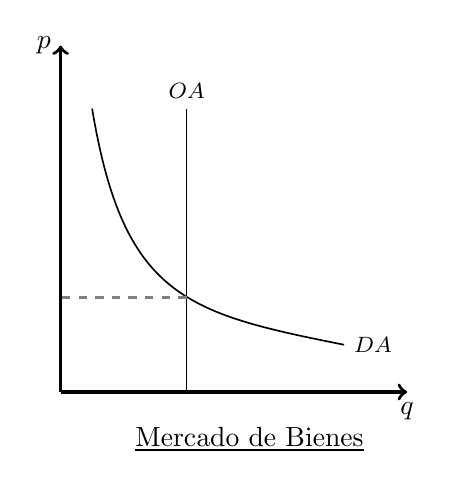
\begin{tikzpicture}[scale=0.4]
                            \draw[very thick,<-] (0,11)--(0,0);
                            \draw[very thick,->] (0,0)--(11,0) node[below]{$q$};
                            \node[left] at (0,11) {$p$};
                            \node[] at(6,-1.5) {\underline{Mercado de Bienes}};
                            \draw[semithick] (1,9).. controls (2,3) and (4, 2.5) .. (9, 1.5) node [right]{\footnotesize $DA$};
                            \draw[semithick](4, 0)--(4, 9) node [above]{\footnotesize $OA$};
                            \draw[thick, gray, dashed] (4,3)--(0,3);
                        \end{tikzpicture}
                    \end{center}
                \end{minipage}
                \begin{minipage}[b]{0.45\textwidth}
                    \begin{center}
                        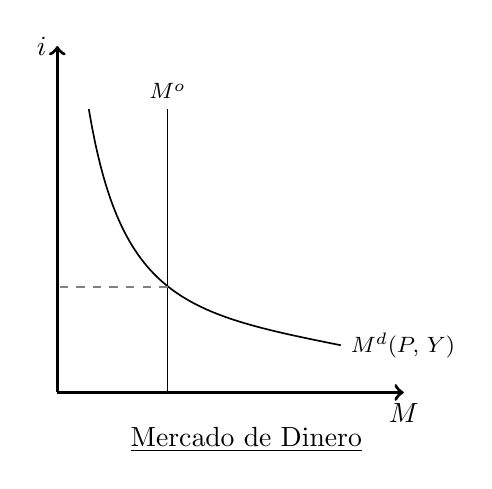
\begin{tikzpicture}[scale=0.4]
                        \draw[very thick,<-] (0,11) node[left]{$i$}--(0,0);
                        \draw[very thick,->] (0,0)--(11,0) node[below]{$M$};
                        \node[right] at (0,11) {};
                        \node[] at(6,-1.5) {\underline{Mercado de Dinero}};
                        \draw[semithick] (1,9).. controls (2,3) and (4, 2.5) .. (9, 1.5) node [right]{\footnotesize $M^{d}(P,\, Y)$};
                        \draw[semithick](3.5, 0)--(3.5, 9) node [above]{\footnotesize $M^{o}$};
                        \draw[thick, gray, dashed] (3.5,3.35)--(0,3.35);
                        \end{tikzpicture}
                    \end{center}
                \end{minipage}
            \end{center}
        \end{figure}
    \end{center} 

\end{frame}

\begin{frame}{El mecano en el mundo keynesiano}
    \begin{center}
    \begin{figure}[H]
    \renewcommand{\figurename}{Figure}
    \begin{center}
    \begin{minipage}[b]{0.45\textwidth}
    \begin{center}
    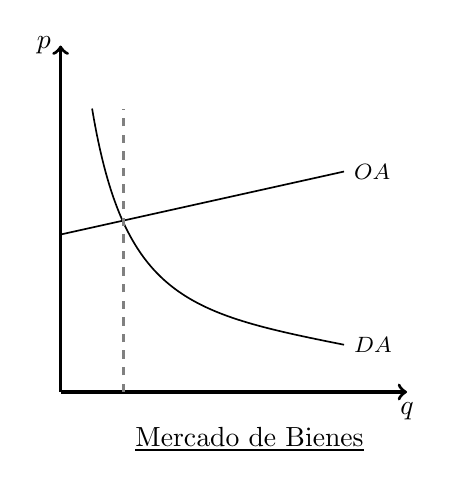
\begin{tikzpicture}[scale=0.4]
    \draw[very thick,<-] (0,11)--(0,0);
    \draw[very thick,->] (0,0)--(11,0) node[below]{$q$};
    \node[left] at (0,11) {$p$};
    \node[] at(6,-1.5) {\underline{Mercado de Bienes}};
    \draw[semithick] (1,9).. controls (2,3) and (4, 2.5) .. (9, 1.5) node [right]{\footnotesize $DA$};
    \draw[semithick](0, 5)--(9,7) node [right]{\footnotesize $OA$};
    \draw[thick, gray, dashed] (2,0)--(2,9);
    \end{tikzpicture}
    \end{center}
    \end{minipage}
    \begin{minipage}[b]{0.45\textwidth}
    \begin{center}
    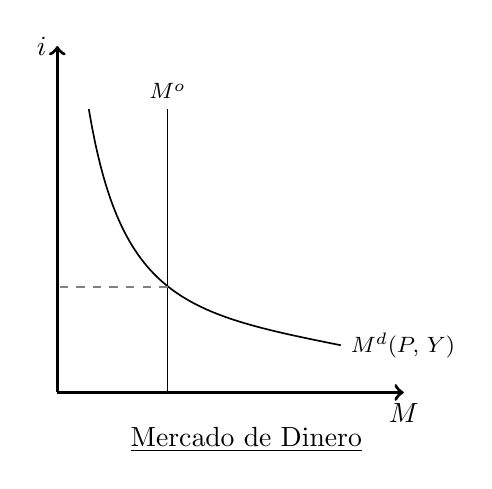
\begin{tikzpicture}[scale=0.4]
    \draw[very thick,<-] (0,11) node[left]{$i$}--(0,0);
    \draw[very thick,->] (0,0)--(11,0) node[below]{$M$};
    \node[right] at (0,11) {};
    \node[] at(6,-1.5) {\underline{Mercado de Dinero}};
    \draw[semithick] (1,9).. controls (2,3) and (4, 2.5) .. (9, 1.5) node [right]{\footnotesize $M^{d}(P,\, Y)$};
    \draw[semithick](3.5, 0)--(3.5, 9) node [above]{\footnotesize $M^{o}$};
    \draw[thick, gray, dashed] (3.5,3.35)--(0,3.35);
    \end{tikzpicture}
    \end{center}
    \end{minipage}
    \end{center}
    \end{figure}
    \end{center} 
\end{frame}

\begin{frame}{Política Monetaria en el mundo clásico}

    \begin{center}
    \begin{figure}[H]
    \renewcommand{\figurename}{Figure}
    \begin{center}
    \begin{minipage}[b]{0.45\textwidth}
    \begin{center}
    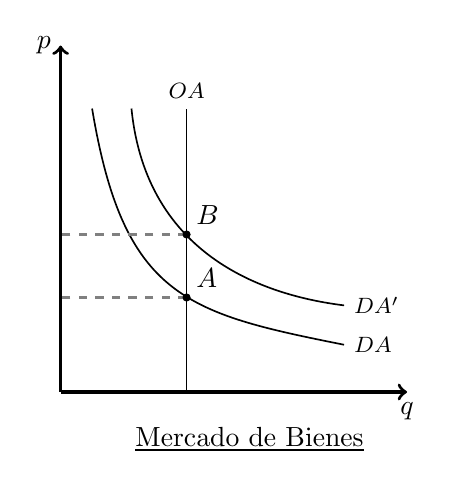
\begin{tikzpicture}[scale=0.4]
    \draw[very thick,<-] (0,11)--(0,0);
    \draw[very thick,->] (0,0)--(11,0) node[below]{$q$};
    \node[left] at (0,11) {$p$};
    \node[] at(6,-1.5) {\underline{Mercado de Bienes}};
    \draw[semithick] (1,9).. controls (2,3) and (4, 2.5) .. (9, 1.5) node [right]{\footnotesize $DA$};
    \draw[semithick] (2.25,9).. controls (2.75,4) and (7, 3) .. (9, 2.75) node [right]{\footnotesize $DA'$};
    \draw[semithick](4, 0)--(4, 9) node [above]{\footnotesize $OA$};
    \draw[thick, gray, dashed] (4,3)--(0,3);
    \draw[thick, gray, dashed] (4,5)--(0,5);
    \draw[fill] (4,3) circle [radius =0.11] node[above right] {$A$}; 
    \draw[fill] (4,5) circle [radius =0.11] node[above right] {$B$}; 
    \end{tikzpicture}
    \end{center}
    \end{minipage}
    \begin{minipage}[b]{0.45\textwidth}
    \begin{center}
    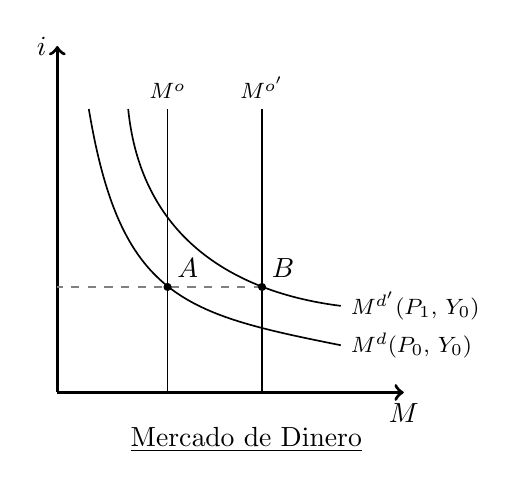
\begin{tikzpicture}[scale=0.4]
    \draw[very thick,<-] (0,11) node[left]{$i$}--(0,0);
    \draw[very thick,->] (0,0)--(11,0) node[below]{$M$};
    \node[right] at (0,11) {};
    \node[] at(6,-1.5) {\underline{Mercado de Dinero}};
    \draw[semithick] (1,9).. controls (2,3) and (4, 2.5) .. (9, 1.5) node [right]{\footnotesize $M^{d}(P_0,\, Y_0)$};
    \draw[semithick] (2.25,9).. controls (2.75,4) and (7, 3) .. (9, 2.75) node [right]{\footnotesize $M^{d'}(P_1,\, Y_0)$};
    \draw[semithick](3.5, 0)--(3.5, 9) node [above]{\footnotesize $M^{o}$};
    \draw[semithick](6.5, 0)--(6.5, 9) node [above]{\footnotesize $M^{o'}$};
    \draw[thick, gray, dashed] (6.5,3.35)--(0,3.35);
    \draw[fill] (3.5,3.35) circle [radius =0.11] node[above right] {$A$}; 
    \draw[fill] (6.5,3.35) circle [radius =0.11] node[above right] {$B$}; 
    \end{tikzpicture}
    \end{center}
    \end{minipage}
    \end{center}
    \end{figure}
    \end{center}
\end{frame}


\begin{frame}{Política monetaria en el mundo clásico}
\begin{itemize}
    \item “Aumenta la demanda agregada” al meter liquidez en el sistema 
    \item Pero el producto está dado por la oferta agregada
    \item Por lo que el aumento en la demanda presiona sobre los precios
    \item Lo que lleva a que los precios aumenten proporcionalmente a lo que aumentó la cantidad de dinero
    \item Oferta y demanda de dinero simplemente se corren para encontrar el equilibrio en el mismo nivel.
    \item $\uparrow M V=\uparrow P Y$ 
    \item Dicotomía clásica (“Neutralidad del dinero”) - $(Y \text{ constante, } M \rightarrow P)$
    \end{itemize}
\end{frame}

\begin{frame}{Política monetaria en el mundo keynesiano}
    \begin{center}
    \begin{figure}[H]
    \renewcommand{\figurename}{Figure}
    \begin{center}
    \begin{minipage}[b]{0.45\textwidth}
    \begin{center}
    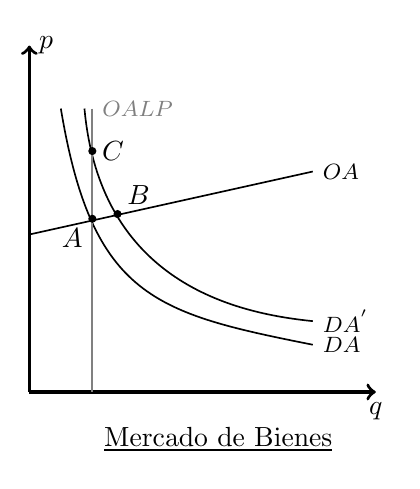
\begin{tikzpicture}[scale=0.4]
    \draw[very thick,<-] (0,11)--(0,0);
    \draw[very thick,->] (0,0)--(11,0) node[below]{$q$};
    \node[right] at (0,11) {$p$};
    \node[] at(6,-1.5) {\underline{Mercado de Bienes}};
    \draw[semithick] (1,9).. controls (2,3) and (4, 2.5) .. (9, 1.5) node [right]{\footnotesize $DA$};
    \draw[semithick] (1.75,9).. controls (2.25,3.5) and (6.5,2.5) .. (9, 2.25) node [right]{\footnotesize $DA^{'}$};
    \draw[semithick](0, 5)--(9, 7) node [right]{\footnotesize $OA$};
    \draw[semithick, gray, fill] (2,0)--(2,9) node [right]{\footnotesize $OALP$};
    \draw[fill] (2,5.5) circle [radius =0.11] node[below left] {$A$}; 
    \draw[fill] (2.8,5.65) circle [radius =0.11] node[above right] {$B$}; 
    \draw[fill] (2,7.65) circle [radius =0.11] node[right] {$C$};
    \end{tikzpicture}
    \end{center}
    \end{minipage}
    \begin{minipage}[b]{0.45\textwidth}
    \begin{center}
    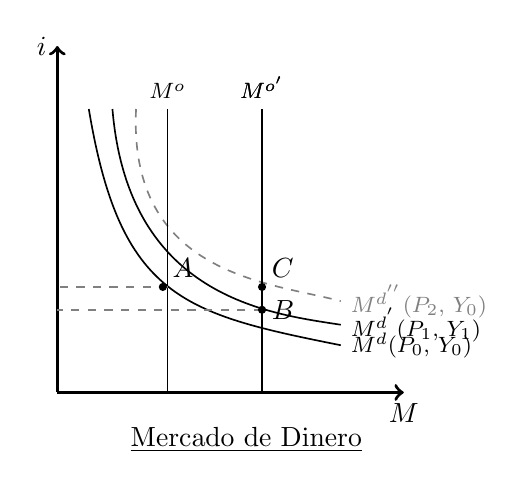
\begin{tikzpicture}[scale=0.4]
    \draw[very thick,<-] (0,11) node[left]{$i$}--(0,0);
    \draw[very thick,->] (0,0)--(11,0) node[below]{$M$};
    \node[right] at (0,11) {};
    \node[] at(6,-1.5) {\underline{Mercado de Dinero}};
    \draw[semithick] (1,9).. controls (2,3) and (4, 2.5) .. (9, 1.5) node [right]{\footnotesize $M^{d}(P_0,\, Y_0)$};
    \draw[semithick] (1.75,9).. controls (2.25,3) and (6.75, 2.5) .. (9, 2.15) node [right]{\footnotesize $M^{d^{'}}(P_1,\, Y_1)$};
    \draw[semithick, gray, dashed] (2.5,9).. controls (2.25,3.7) and (6.75, 3.5) .. (9, 2.9) node [right]{\footnotesize $M^{d^{''}}(P_2,\, Y_0)$};
    \draw[semithick](3.5, 0)--(3.5, 9) node [above]{\footnotesize $M^{o}$};
    \draw[semithick](6.5, 0)--(6.5, 9) node [above]{\footnotesize $M^{o'}$};
    \draw[semithick](6.5, 0)--(6.5, 9) node [above]{\footnotesize $M^{o'}$};
    \draw[semithick, gray, dashed] (3.5,3.35)--(0,3.35);
    \draw[semithick, gray, dashed] (6.5,2.625)--(0,2.625);
    \draw[fill] (3.35,3.35) circle [radius =0.11] node[above right] {$A$}; 
    \draw[fill] (6.5,2.625) circle [radius =0.11] node[right] {$B$}; 
    \draw[fill] (6.5,3.35) circle [radius =0.11] node[above right] {$C$}; 
    \end{tikzpicture}
    \end{center}
    \end{minipage}
    \end{center}
    \end{figure}
    \end{center}   
\end{frame}


\begin{frame}{Política monetaria en el mundo keynesiano}

\begin{itemize}
    \item Ahora “aumenta la demanda agregada” pero ahora esto baja la tasa de interés y lleva a un aumento en el producto.
    \item El dinero excedente reduce la tasa de interés en el mercado de crédito
    \item $\uparrow M V(i) \downarrow=\bar{P} Y \uparrow$
    \item (P constante $, M \rightarrow i, i \rightarrow Y)$
\end{itemize}
 

\end{frame}

\begin{frame}{¿Es efectiva la política monetaria?}

    \begin{itemize}
        \item Depende del contexto si los precios se mueven rápido no va a lograr mucho, si los precios son "rígidos" tendrá más impacto. 
        \item En definitiva es una cuestión de contexto.
        \item Podríamos presumir que la política monetaria en Argentina sería menos efectiva que en los EEUU

    \end{itemize}
    
\end{frame}

\begin{frame}{¿Cómo funciona la política monetaria?}
    
    \centering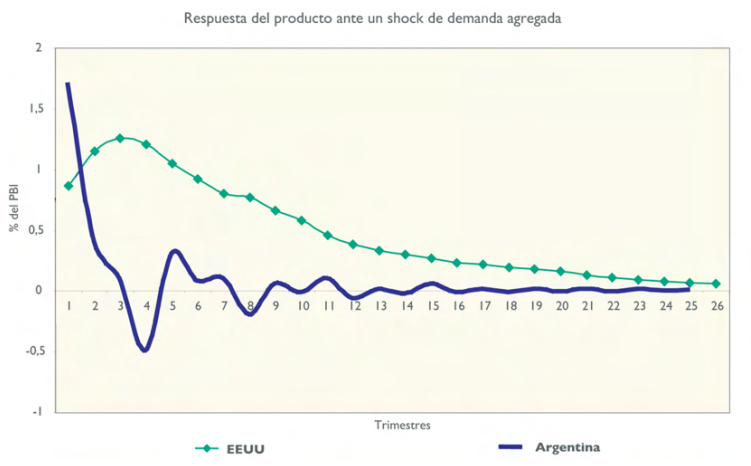
\includegraphics[width=11cm]{../Figures/C40.8.png}\

\end{frame}


\end{document}
